\section{解的检验}
\label{sec:ivp-verification}

经过一番代数整理，得到了$x^2+t^2=1$这样的关系，问题解决了吗？这只是一个等式，还不是一条定义在某个区间上的曲线。在讨论任何求解方法之前，先规定一条曲线要满足什么才算解。

\begin{definition}[经典解]
 \label{def:ivp-classical-solution}
 考虑定义~\ref{def:ivp-ivp}的初值问题。设$I\subseteq T$是包含$t_0$的非退化区间，曲线$\bm{x}:I\to\bm{D}$在$I$的每一点可微（区间端点属于$I$时取单侧导数）。若
 \begin{equation}
 \dot{\bm{x}}(t)=\bm{f}\bigl(t,\bm{x}(t)\bigr)\quad\text{对每个}t\in I\text{成立，}\qquad
 \bm{x}(t_0)=\bm{x}_0,
 \label{eq:ivp-classical-solution}
 \end{equation}
 则称$\bm{x}$是初值问题在$I$上的\term{经典解}（classical solution），其图像称为\term{解曲线}（solution curve）。
\end{definition}

这个定义要求核对四件事。第一，定义域是一个区间，不能是几段分开的时间。第二，$\bm{x}(t)$始终留在$\bm{D}$中，右端处处有定义。第三，方程在区间的每一点成立，不只是在初始时刻。第四，初值成立。若$\bm{f}$连续，复合函数$t\mapsto\bm{f}(t,\bm{x}(t))$也连续，由方程可知$\dot{\bm{x}}$连续，此时经典解自动连续可微。

用这四条来验算式~\eqref{eq:ivp-logistic-solution}。函数$x(t)=\mathrm{e}^{t}/(9+\mathrm{e}^{t})$在整个实轴上有定义，分母恒正，所以取$I=\mathbb{R}$。按商的求导法则，
\[
 \dot{x}(t)=\frac{\mathrm{e}^{t}(9+\mathrm{e}^{t})-\mathrm{e}^{t}\mathrm{e}^{t}}{(9+\mathrm{e}^{t})^2}
 =\frac{9\mathrm{e}^{t}}{(9+\mathrm{e}^{t})^2}.
\]
另一方面，把$x(t)$代入右端，先算$1-x=9/(9+\mathrm{e}^{t})$，于是
\[
 x(1-x)=\frac{\mathrm{e}^{t}}{9+\mathrm{e}^{t}}\cdot\frac{9}{9+\mathrm{e}^{t}}
 =\frac{9\mathrm{e}^{t}}{(9+\mathrm{e}^{t})^2}.
\]
两式相同，方程成立。又$x(0)=1/10$，初值成立。这里$\bm{D}=\mathbb{R}$，取值范围没有限制。

\paragraph{隐式公式需要选支和定区间}
考虑$\dot{x}=-t/x$，$x(0)=1$。这里$T=\mathbb{R}$，右端在$x=0$处没有定义，所以取$D=(0,\infty)$，初值$1$落在其中。把方程写成$x\dot{x}=-t$，两边都是全导数：
\[
 \frac{\mathrm{d}}{\mathrm{d}t}\Bigl(\frac{x^2}{2}\Bigr)=-t.
\]
积分并代入初值，得到隐式关系
\begin{equation}
 x^2+t^2=1.
 \label{eq:ivp-implicit-circle}
\end{equation}

式~\eqref{eq:ivp-implicit-circle}是图~\ref{fig:ivp-implicit-branches}中的整个圆，它在每个$t\in(-1,1)$上有两个$x$，不是一条曲线。初值选中上半支$x=\sqrt{1-t^2}$。在$(-1,1)$上$x>0$，直接求导：
\[
 \dot{x}=\frac{-t}{\sqrt{1-t^2}}=-\frac{t}{x},
\]
方程成立，解的存在区间是$I=(-1,1)$。下半支从$x(0)=-1$出发，属于$D=(-\infty,0)$上的另一个初值问题，不能接在上半支后面。

\begin{BookInlineFigure}
 \centering
 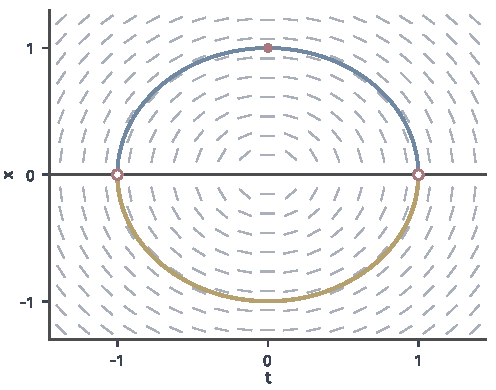
\includegraphics[width=84mm]{figures/06-differential-equations/01-ordinary-differential-equations/matplotlib/ivp-implicit-branches/figure.pdf}
 \caption{$\dot{x}=-t/x$的隐式解$x^2+t^2=1$。深灰色直线$x=0$上右端没有定义，把平面分成两部分。红点是初值$x(0)=1$，它选中蓝色上半支；黄色下半支是另一个初值问题的解。空心点处切线竖直，解不能延伸到端点$t=\pm 1$。}
 \label{fig:ivp-implicit-branches}
\end{BookInlineFigure}

端点$t=\pm 1$也不属于存在区间。那里$x=0$，已经离开了$D$；从公式看，$\sqrt{1-t^2}$在$t=\pm 1$的导数也不存在。解的存在区间比公式的“定义范围”$[-1,1]$小，这正是定义中第二条和第三条要求的结果。

\paragraph{平衡解}
第二种容易被漏掉的解是常值解。对$\dot{x}=x(1-x)$，右端在$x=0$和$x=1$处为零，所以常值函数$x\equiv 0$和$x\equiv 1$满足方程：左边的导数为零，右边也为零。

一般地，若$\bm{x}^{\star}\in\bm{D}$对每个$t\in T$都满足$\bm{f}(t,\bm{x}^{\star})=\bm{0}$，则常值曲线$\bm{x}(t)\equiv\bm{x}^{\star}$是从$\bm{x}^{\star}$出发的解，称为\term{平衡解}（equilibrium solution）。它的存在区间是整个$T$。第~\ref{sec:ivp-separable}小节的求解过程要除以右端的因子，平衡解正好落在被除掉的位置。例如式~\eqref{eq:ivp-logistic}的非平衡解可以用一个常数$C$统一写成下面的公式，这样的公式称为\term{通解}（general solution）：
\[
 x(t)=\frac{1}{1+C\mathrm{e}^{-t}},
\]
$C=0$给出$x\equiv 1$，但没有任何有限的$C$能给出$x\equiv 0$。用通解公式来核对“解是否都找到了”时，这样的解需要单独列出。

\paragraph{有限时间爆炸}
第三种现象是公式本身完全正常，解却走不到远处。考虑$\dot{x}=x^2$，$x(0)=1$。曲线$x(t)=1/(1-t)$的导数是
\[
 \dot{x}(t)=\frac{1}{(1-t)^2}=x(t)^2,
\]
并且$x(0)=1$。这是经典解，但它只在$t<1$时有意义：当$t$从左侧趋于$1$时，$x(t)\to+\infty$。这种现象称为\term{有限时间爆炸}（finite-time blow-up）。

右端$x^2$是处处光滑的函数，没有任何奇异之处，爆炸完全来自增长本身。翻倍时间可以说明它和指数增长的差别。由解的公式，$x_0=1$的解到达高度$x$的时刻是$t=1-1/x$。于是从$x=a$涨到$x=2a$需要的时间是
\[
 \frac{1}{2a}=\Bigl(1-\frac{1}{2a}\Bigr)-\Bigl(1-\frac{1}{a}\Bigr).
\]
从$1$开始，依次翻倍所需时间是$1/2,1/4,1/8,\ldots$，总和是$1$，这正是爆炸时刻。指数增长$\dot{x}=x$每次翻倍都需要$\ln 2$的时间，翻倍无穷多次要无穷长的时间。

\begin{BookInlineFigure}
 \centering
 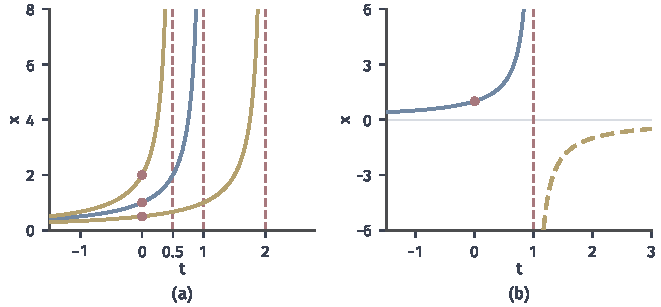
\includegraphics[width=112mm]{figures/06-differential-equations/01-ordinary-differential-equations/matplotlib/ivp-blow-up/figure.pdf}
 \caption{$\dot{x}=x^2$的有限时间爆炸。(a)初值$x_0=1$（蓝）与$x_0=0.5,\,2$（黄）的解$x=x_0/(1-x_0t)$，红色虚线是爆炸时刻$1/x_0$。初值越大，爆炸越早。(b)公式$1/(1-t)$在$t>1$还有一支（黄色虚线），它与蓝线被$t=1$隔开，也不经过初值，不属于这个初值问题的解。}
 \label{fig:ivp-blow-up}
\end{BookInlineFigure}

对一般初值$x_0>0$，解是$x=x_0/(1-x_0t)$，存在区间是$(-\infty,1/x_0)$，图~\ref{fig:ivp-blow-up}(a)显示爆炸时刻依赖于初值。这是非线性方程的特点：同一个方程，不同初值的解活得长短不同，存在区间事先无法从方程上直接读出来。

公式$1/(1-t)$在$t>1$时也有值，而且也满足微分等式。但图~\ref{fig:ivp-blow-up}(b)中右侧的那一支从负无穷升上来，与初值所在的那一支被$t=1$隔开，不在同一个区间上，所以不是我们的解。“解的存在区间是区间”这一要求在这里起作用。

\paragraph{检查清单}
把上面三个例子收拢起来。拿到一个候选公式时，依次回答下表中的问题；前两行决定存在区间，后两行决定它确实是解。

\begin{BookInlineTable}
 \centering
 \caption{候选解的检查项}
 \label{tab:ivp-checklist}
 \begin{tabular}{ll}
 \toprule
 检查项 & 对应的例子 \\
 \midrule
 是否是定义在一个区间上的函数 & 圆$x^2+t^2=1$要选支 \\
 状态是否留在右端的定义域内 & $\dot{x}=-t/x$要求$x\neq 0$ \\
 该区间内的每一点方程是否成立 & $1/(1-t)$只取$t<1$的一支 \\
 初值是否成立，是否漏掉平衡解 & $x\equiv 0$不在通解公式中 \\
 \bottomrule
 \end{tabular}
\end{BookInlineTable}

这张表只用来检验一条给定的曲线。它不回答“还有没有别的解”，也不回答“解最长能延伸到哪里”，这两个问题由第~\ref{chap:ode-existence-continuation}章回答。
